\documentclass{article}


\usepackage[margin=0.6in]{geometry}
\usepackage{amssymb, amsmath, amsfonts}
\usepackage{tabularx}
\usepackage{arydshln}
\usepackage{mathtools}
\usepackage{cancel}
\usepackage{physics}
\usepackage{enumerate}
\usepackage{placeins}
\usepackage{enumitem}
\usepackage{nth}
\usepackage{array}
\usepackage{tikz}
\usepackage{nicefrac}
\usepackage{pgfplots}
\newcommand{\enth}{$n$th}
\newcommand{\Rl}{\mathbb{R}}
\newcommand{\Cx}{\mathbb{C}}
\newcommand{\sgn}[1]{\text{sgn}\qty[#1]}
\newcommand{\ran}[1]{\text{ran}\qty[#1]}
\newcommand{\E}{\varepsilon}
\newcommand{\qiq}{\qquad \implies \qquad}
\newcommand{\half}{\nicefrac{1}{2}}
\newcommand{\third}{\nicefrac{1}{3}}
\newcommand{\quarter}{\nicefrac{1}{4}}
\newcommand{\f}[3]{#1\ :\ #2 \rightarrow #3}

\newcommand{\tridsym}[3]{
    \qty(\begin{array}{ccccc}
                    #1 & #2 & & & \\
                    #3 & #1 & #2 & & \\
                    & \ddots & \ddots & \ddots &  \\
                    & & #3 & #1 & #2 \\
                    & & & #3 & #1
                \end{array})
}


\DeclareMathOperator*{\esssup}{\text{ess~sup}}

\title{MAT 228A Notes}
\author{Sam Fleischer}
\date{November 8, 2016}

\begin{document}
    \maketitle

    \section{$\omega$-Jacobi in 1D}
        Over/under relaxation in GS leads to SOR.  What happens when we add a parameter to Jacobi method?
        \begin{itemize}
            \item
                $u_j^{k+1} = \nicefrac{\omega}{2}\qty(u_{j-1}^k + u_{j+1}^k - ?) + \qty(1 - \omega)u_j^k$
            \item
                Update matrix is $\omega T_J + (1 - \omega)I$ where $T_J$ is the update matrix of the Jacobi method.  The eigenvalues are rescaled and shifted from the eigenvalues of $T_J$.  Eigenvectors are
                \begin{align*}
                    u_{j,\ell} = \sin(\ell\pi x_j)
                \end{align*}
                Eigenvalues are
                \begin{align*}
                    \mu_\ell = \omega\cos(\ell\pi h) + (1 - \omega)
                \end{align*}
            \item
                For $\omega = 1$, we get
                \begin{figure}[ht!]
                    \centering
                    \begin{tikzpicture}[scale=0.6]
                        \begin{axis}[ylabel style={rotate=-90},xlabel={$\theta$},ylabel={$\mu_n^k$},ymin=-1.2,xmin=0,xmax=pi]
                            \addplot[domain=0:pi,black]{cos(deg(x))};
                            \addplot[domain=-10:10,dotted]{0};
                        \end{axis}
                    \end{tikzpicture}
                \end{figure}
                \FloatBarrier
                We see slow damping of the low and high frequencies, but rapid damping of the mid frequencies.  For $k = 1$,
                \begin{align*}
                    \mu_1 = \omega\qty(1 - \frac{\pi^2 h^2}{2} + \dots) + \qty(1 - \omega) \approx 1 - \omega\frac{\pi^2h^2}{2}
                \end{align*}
                For $k = n$, 
                \begin{align*}
                    \mu_n =  1 - 2\omega + (\text{higher order terms})
                \end{align*}
                This tells us $\omega \leq 1$ for convergence ($\omega = 1$ is fine when you consider the higher order terms).  And $\omega \geq 0$ in order for $\mu_1$ to converge.
            \item
                For $\half<\omega<1$ we get
                \begin{figure}[ht!]
                    \centering
                    \begin{tikzpicture}[scale=0.6]
                        \begin{axis}[ylabel style={rotate=-90},xlabel={$\theta$},ylabel={$\mu_n^k$},ymin=-1.2,xmin=0,xmax=pi]
                            \addplot[domain=0:pi,black]{0.6*cos(deg(x)) + 0.4};
                            \addplot[domain=-10:10,dotted]{0};
                        \end{axis}
                    \end{tikzpicture}
                \end{figure}
                \FloatBarrier
                The big idea of multigrid is to combine smoothing and coarse grid.
        \end{itemize}

    \section{Choosing $\omega$ to wipe out the highest frequencies}
        Choosing $\omega = \half$ gives us
        \begin{figure}[ht!]
            \centering
            \begin{tikzpicture}[scale=0.6]
                \begin{axis}[ylabel style={rotate=-90},xlabel={$\theta$},ylabel={$\mu_n^k$},ymin=-1.2,xmin=0,xmax=pi]
                    \addplot[domain=0:pi,black]{0.5*cos(deg(x)) + 0.5};
                    \addplot[domain=-10:10,dotted]{0};
                \end{axis}
            \end{tikzpicture}
        \end{figure}
        \FloatBarrier
        $\omega=\half$ is most effective on highest frequencies.  We want to reduce frequencies with wave greater than or equal to $\nicefrac{n}{2}$.  This gets rid of the highest frequencies but made convergence of midrange fequencies much worse.  What value of $\omega$ is optimal to reduce high-range frequencies?
        \begin{figure}[ht!]
            \centering
            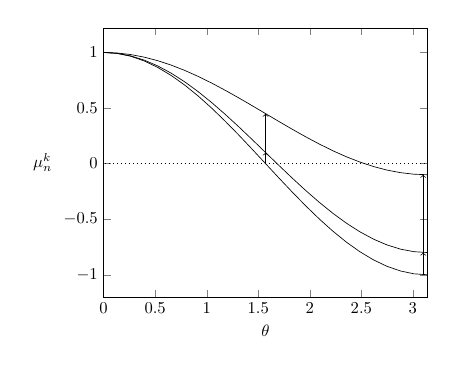
\begin{tikzpicture}[scale=0.6]
                \begin{axis}[ylabel style={rotate=-90},xlabel={$\theta$},ylabel={$\mu_n^k$},ymin=-1.2,xmin=0,xmax=pi]
                    \addplot[domain=0:pi,black]{0.9*cos(deg(x)) + 0.1};
                    \addplot[domain=0:pi,black]{0.55*cos(deg(x)) + 0.45};
                    \addplot[domain=0:pi,black]{cos(deg(x))};
                    \addplot[domain=-10:10,dotted]{0};
                    \addplot[->] coordinates{(pi/2,0) (pi/2,0.1)};
                    \addplot[->] coordinates{(pi/2,0.1) (pi/2,0.45)};
                    \addplot[->] coordinates{(3.1,-1) (3.1,-0.8)};
                    \addplot[->] coordinates{(3.1,-0.8) (3.1,-0.1)};
                \end{axis}
            \end{tikzpicture}
        \end{figure}
        \FloatBarrier
        $\omega_\text{opt}$ is the omega which makes
        \begin{align*}
            \omega_\text{opt}\cos(\ell\pi N) + (1 - \omega_\text{opt}) = -\qty[\omega_\text{opt}\cos(\ell\pi \frac{N}{2}) + (1 - \omega_\text{opt})]
        \end{align*}
        So we want $1 - \omega^* = 1 - 2\omega^*$, i.e.~$\omega^* = \nicefrac{2}{3}$, so we get $\mu^* = 1 - \omega^* = \third$.  So all mid-high level frequencies are reduced by a factor of $e$ per iteration.  Just 2 iterations reduces error by approximately an order of magnitude.  Set $\mu$ equal to
        \begin{align*}
            \mu \coloneqq \max_{\nicefrac{n}{2}\leq k \leq n}\abs{\mu_k}
        \end{align*}
        $\mu$ is called the smoothin factor.  It is the largest factor by which the high frequency ($k \geq \nicefrac{n}{2}$) modes are reduced with one application of the smoother.
        \subsection{Smoothing Factors in multiple dimensions..}
            \begin{align*}
                \begin{array}{||c|c|c|c|c||} \hline\hline
                    & \omega^* & \mu_{\omega-\text{Jacobi}} & \mu_{\text{GS-lex}} & \mu_{\text{GS-RB}} \\\hline
                    \text{1D} & \nicefrac{2}{3} & \third & 0.45 & 0.125 \\\hline
                    \text{2D} & \nicefrac{4}{5} & \nicefrac{3}{5} & 0.5 & 0.25 \\\hline
                    \text{3D} & \nicefrac{6}{7} & \nicefrac{5}{7} & 0.567 & 0.445 \\\hline\hline
                \end{array}
            \end{align*}
            Clearly GS-RB is the winner in higher dimensions.

    \FloatBarrier
    \section{GS-Lex analysis of smoothing}
        Eigenvectors of the iteration matrix are not $\sin$ waves.
        
        \subsection{Local Fourier Analysis}
            Lets ignore boundaries and analyze the problem on the infinite domain.  We still have a discrete domain but it is the whole real line:
            \begin{align}
                x_j = jh \qquad j \in \mathbb{Z}
            \end{align}
            The eigenfunctions are of the form
            \begin{align}
                u_\ell^k = \exp(ikx_\ell)
            \end{align}
            What values does $k$ take?  Using duality of the Fourier transform, we know that the highest $k$ corresponds to
            oscillations between $1$ and $-1$ at each grid point.  It has period $2h$.  So $k_\text{max}h = \pi$.  $k_\text{max} = \nicefrac{\pi}{h}$.  Thus
            \begin{align}
                -\frac{\pi}{h} < k \leq \frac{\pi}{h}
            \end{align}
            are the meaningful values of $k$, that is
            \begin{align}
                -\pi < kh \leq \pi
            \end{align}
            but let $\theta \coloneqq kh$, so
            \begin{align}
                -\pi < \theta \leq \pi
            \end{align}
            That is, $\theta$ is the continuous wave number.  So,
            \begin{align}
                u_\ell(\theta) = \exp[ikx_\ell] = \exp[ikh\ell] = \underbrace{\exp[i\theta\ell]}_\text{continuoum of eigenfunctions}
            \end{align}
            since $x_\ell = h\ell$ and $kh = \theta$.  We have a bounded continuous spectrum. \\

            Let's define high-frequency as $\nicefrac{\pi}{2} \leq \abs{\theta} \leq \pi$.  What is the worst eigenvalue? \\

            \subsection{GS error}
                \begin{align}
                    e^{k+1} = Te^k
                \end{align}
                \begin{align}
                    e_\ell^{k+1} = \frac{1}{2}\qty(e_{\ell-1}^{k+1} + e_{\ell+1}^{k})
                \end{align}
                Fix $\theta$..
                \begin{align}
                    e^k = \exp(i\ell\theta) \\
                    \implies e^{k+1} = Te^k = ae^k
                \end{align}
                where $a$ is called the amplification factor (the eigenvalue).  So we get
                \begin{align}
                    ae_\ell^k &= \frac{1}{2}\qty(ae_{\ell+1}^k + e_{\ell+1}^k) \\
                    e_{\ell-1} &= e_\ell\exp(-i\theta) \\
                    e_{\ell+1} &= e_\ell\exp(i\theta) \\
                    \implies a &= \frac{1}{2}\qty(a\exp(-i\theta) + \exp(i\theta)) \\
                    \implies a &= \frac{\exp(i\theta)}{2 - \exp(-i\theta)}
                \end{align}
                The smoothing factor
                \begin{align}
                    \mu = \max_{\abs{\theta} \geq \nicefrac{\pi}{2}}\abs{a(\theta)} = \frac{1}{\sqrt{5}} \approx 0.45
                \end{align}
                $\abs{a}$ as a function of $\theta$ that looks kind of Gaussian.

\end{document}



















